\section{Simulation Analysis}
\label{sec:simulation}

\par A simulation analysis was produced in order to better predict the behaviour of the circuit. The used script resorted to the OP-AMP model provided previously to the class and then few modifications were made to produce the final circuit.

\par Starting with the frequency response of the output voltage and phase in the pass band, we have:

\begin{figure}[h] \centering
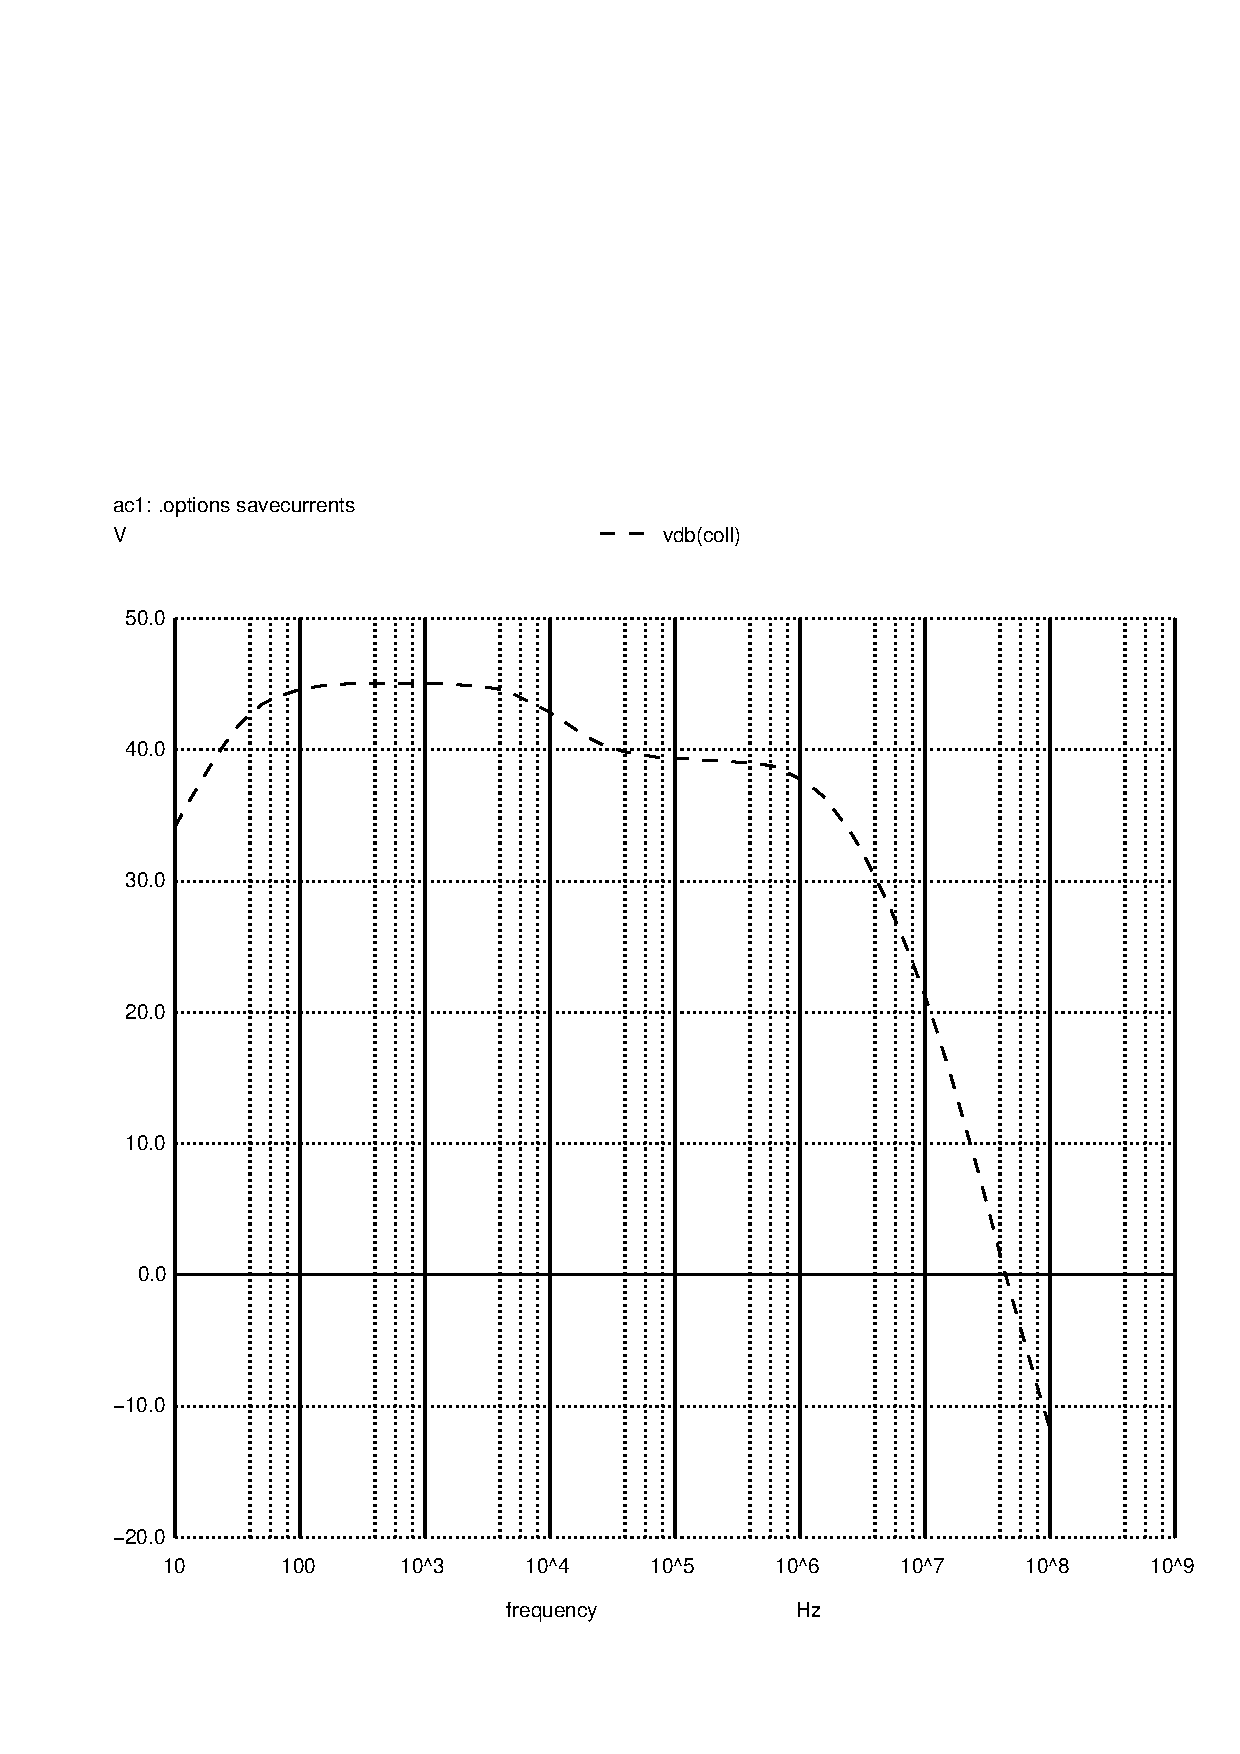
\includegraphics[width=0.6\linewidth]{../sim/vo1f.pdf}
\caption{Frequency response - Output voltage.}
\label{fig:f1}
\end{figure}

\begin{figure}[h] \centering
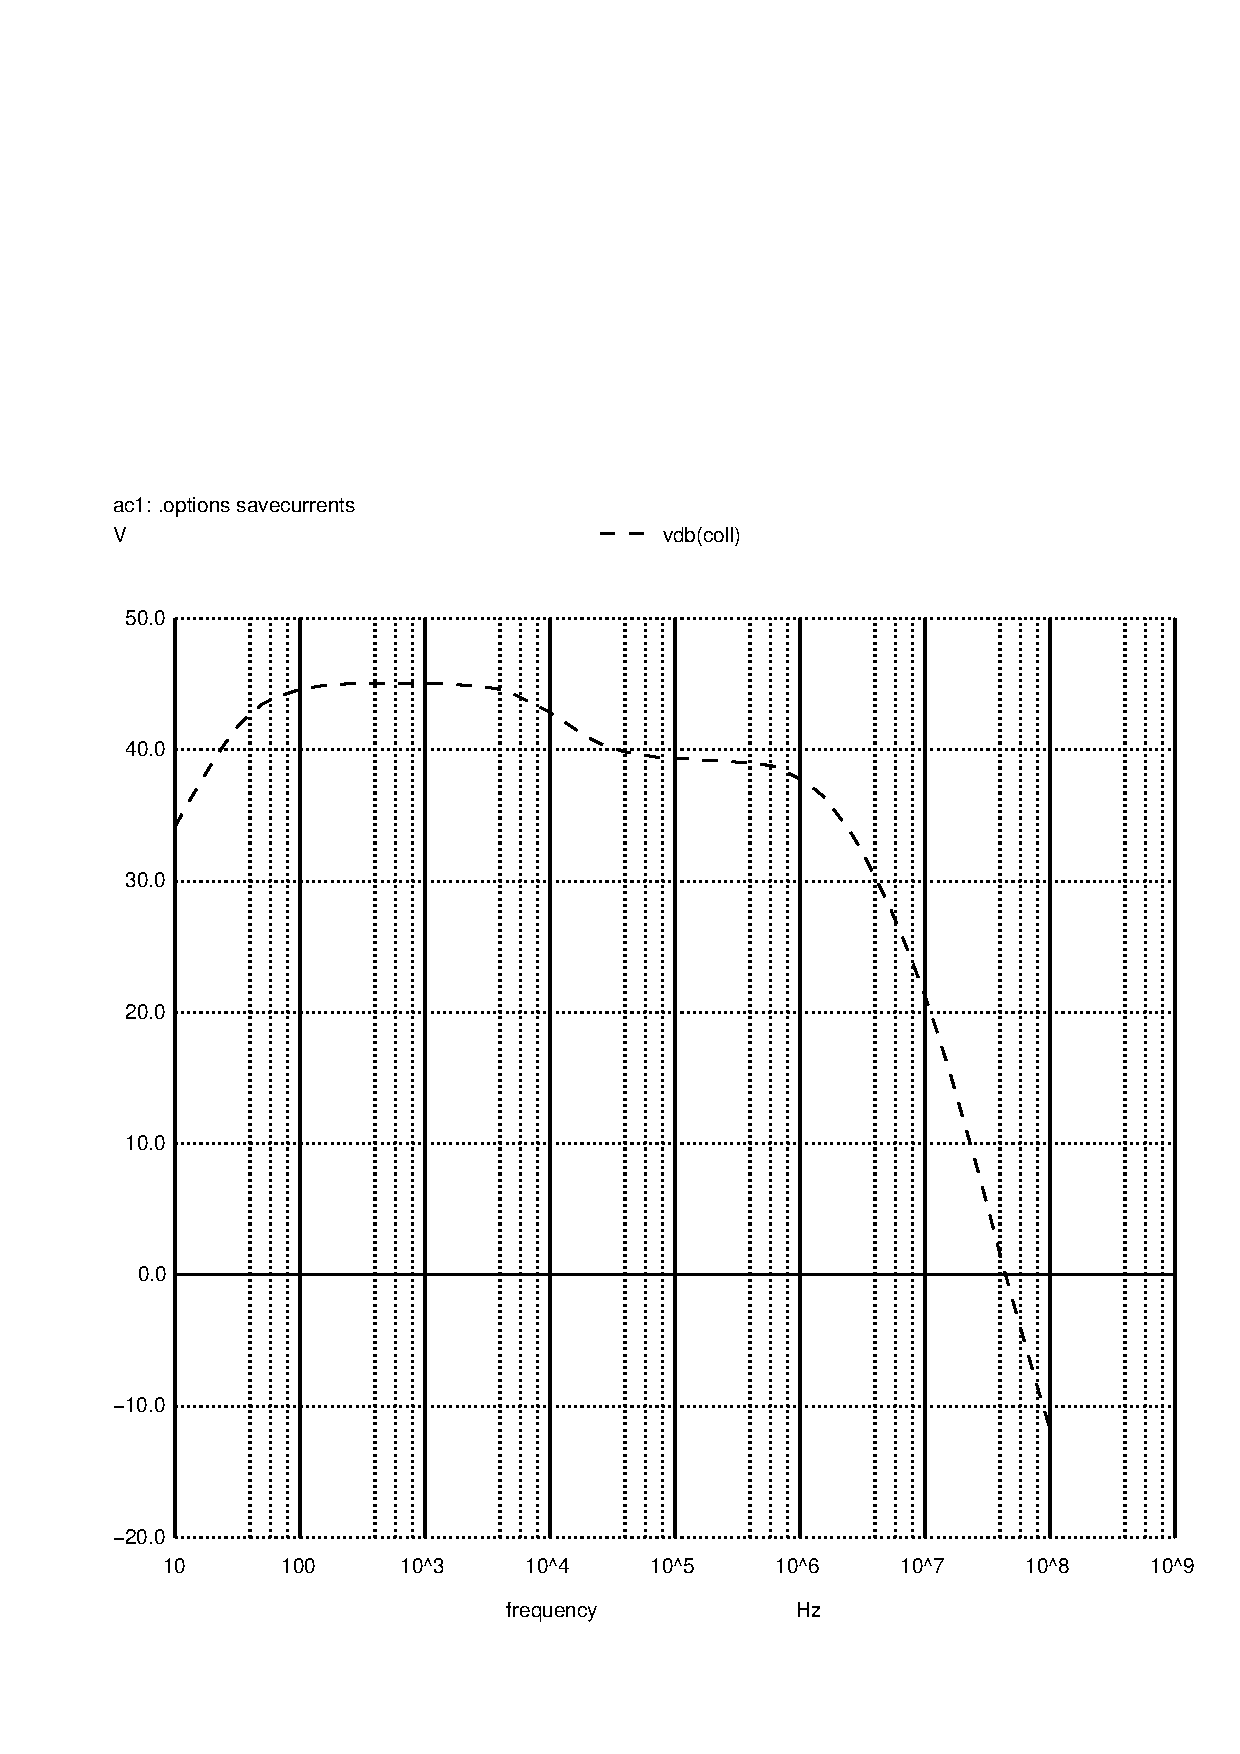
\includegraphics[width=0.6\linewidth]{../sim/vo2f.pdf}
\caption{Frequency response - Phase.}
\label{fig:f2}
\end{figure}

\newpage

\par By a frequency analysis, we were able to determine the low and high cut-off frequencies and, consequently, the central frequency. The following table shows these results and also the gain at the central frequency:

\begin{table}[h]
  \centering
  \begin{tabular}{|l|r|}
    \hline    
   \input{../sim/frs_tab}
   \end{tabular}
  \caption{Frequency results.}
    \label{tab:frs}
\end{table}

\par Then, using the Ngspice tool, the input and output impedances were obtained:

\begin{table}[h]
  \centering
  \begin{tabular}{|l|r|}
    \hline    
   \input{../sim/Zin_tab}
   \end{tabular}
  \caption{Input Impedance.}
    \label{tab:zin}
\end{table}

\newpage

\begin{table}[h]
  \centering
  \begin{tabular}{|l|r|}
    \hline    
    {\bf Name} & {\bf Value}\\ \hline
    \input{../sim/zout_tab}
  \end{tabular}
  \caption{Output Impedance.}
  \label{tab:zout}
\end{table}


\par In the introduction, a formula for the merit of the circuit was given, depending on the cost, gain and central frequency deviations (in relation to the values given by the teacher). Finally, the values for these quantities were simulated, resulting in the next table:

\begin{table}[h]
  \centering
  \begin{tabular}{|l|r|}
    \hline    
    {\bf Name} & {\bf Value}\\ \hline
    \input{../sim/results_tab}
  \end{tabular}
  \caption{Simulated Results.}
  \label{tab:finalr}
\end{table}

\newpage

